
\setchapterpreamble[u]{\margintoc}
\chapter[Er3+ spin coupled to a microwave resonator]{\Er spin coupled to a cavity}
\labch{spins_coupled_to_a_cavity}

\begin{quote}
\itshape

In this chapter we introduce the required techniques used to achieve single spin resolution in our measurements. 
Our detection scheme is based on single microwave photon counting using a detector that is designed and fabricated in-house.
By inductively coupling the \Er spins to a superconducting resonator we enhance the radiative decay rate of the spins via the Purcell effect, which allows the extraction of microwave fluorescence from the spins after a resonant excitation. These photons are routed to the detector where they are readout.

We begin with a discussion of a superconducting circuit inductively coupled to an \Er spin, with the objective of arriving to a quantitative description of the Purcell effect. We then follow with a qualitative description of the detector and its performance metrics.

\end{quote}

\section{Quantum circuits}
\labsec{quantum_circuits}

We consider a lumped element resonator, where the capacitance $C$ and the inductance $L$ can be considered as separate elements (see \reffig{resonator}). Classically, the energy of the system is given by the voltage $V$ that accumulates on the capacitor and the current $I$ that goes through the inductor 

\begin{equation}
    E = \frac{1}{2}LI^2 + \frac{1}{2}CV^2
\end{equation}

This results in a resonant frequency $\omega_r=1/\sqrt{LC}$ with an impedance of $Z_r = \sqrt(L/C)$, and the Hamiltonian of the classical system is 

\begin{equation}
    H_r =\frac{Q^2}{2C} + \frac{\phi^2}{2L}, 
\end{equation}

where $Q$ is the charge on the capacitor and $\phi$ is is the flux of the inductor\sidenote{The charge and flux are related to the voltage and current as 
\begin{align*}
    &I = -\frac{dQ}{dt} = -C\frac{dV}{dt}, \\
    &V = \frac{d\phi}{dt} = L\frac{dI}{dt}
\end{align*}
} the quantization of this Hamiltonian is performed by replacing with the charge and phase operators ($\hat{Q}$ and $\hat{\phi}$) which follow the following commutation relation: $[\hat{Q}, \hat{\phi}]=i\hbar$. By introducing the creation and anihilation operators ($\hat{a}$ and $\hat{a}^\dagger$) we can write the Hamiltonian of the resonator in second quantization


\begin{marginfigure}
    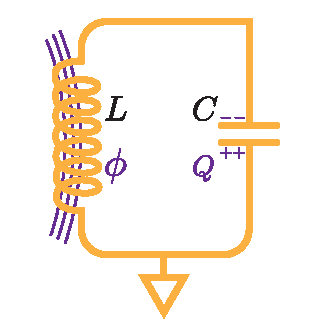
\includegraphics{chapter2/figures/resonator.pdf}
    \caption[Lumped element resonator]{Sketch of a lumped element resonator. The capacitor is defined by the capacitance to ground $C$ and the charge accumulated $Q$ while the inductor by its inductance to ground $L$ and the flux threading the loops $\phi$.}
    \labfig{resonator}
\end{marginfigure}



\begin{align}
\begin{split}
    \cH{r} = \hbar \omega_r(\hat{a}^\dagger \hat{a} + 1/2), \\
    \hat{\phi} = \sqrt{\frac{\hbar Z_r}{2}} (\hat{a}^\dagger + \hat{a}) = \delta \hat{\phi} (\hat{a}^\dagger + \hat{a}), \\
    \hat{Q} = i \sqrt{\frac{\hbar}{2 Z_r}} (\hat{a}^\dagger - \hat{a}) = i \delta \hat{Q} (\hat{a}^\dagger - \hat{a}),
\end{split}
\end{align}

\noindent and the eigenstates of the system are the Fock states $\ket{n}$ with associated energy $\cH{r}\ket{n} = \hbar \omega_r (n + 1/2)$. The potential as a function of the flux and the energy diagram are represented in \reffig{resonator_energy}. The Zero Point Fluctuations (ZPF) of the phase and the charge inside of the resonator ($\delta \hat{\phi}$ and $\delta \hat{Q}$) correspond the root mean square vacuum fluctuations of these quantities. Similarly, the electric and magnetic field generated by the resonator will be given by

\begin{marginfigure}
    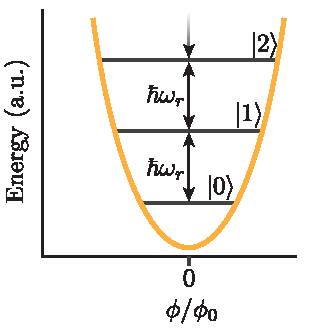
\includegraphics{chapter2/figures/resonator_energy.pdf}
    \caption[Energy of a harmonic oscillator]{Energy diagram (black) and potential (green) of a harmonic oscillator with $\phi_0=  h/2e$. The levels are all separated by $\hbar\omega_r$}
    \labfig{resonator_energy}
\end{marginfigure}

\begin{align}
\begin{split}
    \mathbf{B}(\mathbf{r}) =   \boldsymbol{\delta}\mathbf{B}(\mathbf{r}) \, (\hat{a}^\dagger + \hat{a}), \\
    \mathbf{E}(\mathbf{r}) = i \boldsymbol{\delta}\mathbf{E}(\mathbf{r}) \, (\hat{a}^\dagger + \hat{a}). 
\end{split}
\end{align}

The electric and magnetic field have their associated ZPF ($\boldsymbol{\delta}\mathbf{E}(\mathbf{r})$ and $\boldsymbol{\delta}\mathbf{B}(\mathbf{r})$). These quantities have a spatial distribution: the magnetic field ZPF will be located close to the inductor and the electric field ZPF will be stronger between the capacitor plates.


Throughout this work, the thermal energy of the system $k_B T$ is constantly lower than the energy of the resontor $\hbar \omega_r$ which ensures its quantum nature. 

\section{A spin inductively coupled to a resonator}
\labsec{spin_coupled_to_resonator}


Since the \Er spins are intrinsic magnetic dipoles, they couple inductively to the resonator. Without loss of generality, the Hamiltonian that models the interaction between the two can be written as 

\begin{align}
    \cH{r-s} = \hbar\omega_r(\hat{a}^\dagger \hat{a} + 1/2) +  \omega_S S_z + \cH{int},
\end{align}

\noindent where $\omega_S = | \mathbf{B_0} \cdot \bar{\bar{\gamma}}_{\text{\Er}} | $ is the Larmor frequency of the \Er and we have arbitrarily chosen the $z$-axis as the orientation of $B_0$. The interaction Hamiltonian will be proportional to the magnetic field $\mathbf{B_1}$, generated by the resonator at the spin's position,

\begin{equation}
    \cH{int} = \mathbf{B_1} \cdot \bar{\bar{\gamma}}_{\text{\Er}} \cdot \mathbf{S} = (\hat{a}^\dagger + \hat{a}) \, \boldsymbol{\delta}\mathbf{B} \cdot \bar{\bar{\gamma}}_{\text{\Er}} \cdot \mathbf{S},
\end{equation}

\noindent where $\boldsymbol{\delta}\mathbf{B}$ are the zero-point fluctuations of the magnetic field at the \Er spin's position. The Hamiltonian can be re-formulated in terms of the raising and lowering operators \sidenote{Which are defined as
\begin{align*}
    \hat{S}_+ = \hbar \ket{\Uparrow}\bra{\Downarrow}, \\ 
    \hat{S}_- = \hbar \ket{\Downarrow}\bra{\Uparrow}.
\end{align*}
},

\begin{equation}
    \labeq{res_spin_inter}
    \cH{int} = \hbar (\hat{a}^\dagger + \hat{a}) \, (g_0 \hat{S}_+ + g_0 \hat{S}_- + \alpha_\Downarrow \ket{\Downarrow}\bra{\Downarrow} + \alpha_\Uparrow \ket{\Uparrow}\bra{\Uparrow}), 
\end{equation}

\noindent where $g_0$ is the coupling strength between the resonator and the spin and $\alpha_\Uparrow$ and $\alpha_\Uparrow$ are re-normalization of the energy levels of the electron spin states, given by

\begin{align}
\begin{split}
    g_0 =&\, \bra{\Uparrow} \boldsymbol{\delta}\mathbf{B} \cdot \bar{\bar{\gamma}}_{\text{\Er}} \cdot \mathbf{S} \ket{\Downarrow}, \\ 
    \alpha_\Uparrow =&\, \bra{\Uparrow} \boldsymbol{\delta}\mathbf{B} \cdot \bar{\bar{\gamma}}_{\text{\Er}} \cdot \mathbf{S} \ket{\Uparrow}, \\ 
    \alpha_\Downarrow =&\, \bra{\Downarrow} \boldsymbol{\delta}\mathbf{B} \cdot \bar{\bar{\gamma}}_{\text{\Er}} \cdot \mathbf{S} \ket{\Downarrow}.
\end{split}
\end{align}

The relative strength between the parameters is controlled by the orientation of $\mathbf{B_1}$ with respect to the quantization axis of the \Er ion, $g_0$ is maximized when they are perpendicular to each other and zero when parallel. The effect of this interaction is more easily understood in the rotating frame of the resonator and the spin. The unitarty transformation to this frame is given by

\begin{align}
    \hat{U}(t) = \exp{i\left(\hbar\omega_r(\hat{a}^\dagger \hat{a} + 1/2) +  \omega_S S_z\right)t/\hbar},
\end{align}

\noindent and the Hamiltonian will be transformed as

\begin{align}
\begin{split}
    \cH{r-s}' &= \hat{U}(t) \cH{r-s} \hat{U}^\dagger(t) + \dot{\hat{U}}(t)^\dagger  \hat{U}^\dagger(t) = \hat{U}(t) \cH{int} \hat{U}^\dagger(t) = \\
    &= g_{0} \Big( \hat{a}\hat{S}_{+} e^{i(\omega_{s}-\omega_{r})t} + \hat{a}^{\dagger}\hat{S}_{-} e^{-i(\omega_{s}-\omega_r)t} \Big) \\
    &\quad + g_{0} \Big(\hat{a}\hat{S}_{-} e^{-i(\omega_{s}+\omega_{r})t} + \hat{a}^{\dagger}\hat{S}_{+} e^{i(\omega_{s}+\omega_r)t} \Big) \\
    &\quad + \hbar \big( \hat{a} e^{-i\omega_{r}t} + \hat{a}^{\dagger} e^{i\omega_rt} \big) 
    \big( \alpha_{g}\ket{\Uparrow} \ket{\Downarrow} + \alpha_{e} \ket{\Downarrow} \bra{\Uparrow} \big) \\
    &\sim g_{0} \Big( \hat{a}\hat{S}_{+} e^{i(\omega_{s}-\omega_r)t} 
    + \hat{a}^{\dagger}\hat{S}_{-} e^{-i(\omega_{s}-\omega_r)t} \Big).
\end{split}
\end{align}

The last step corresponds to the rotating-wave approximation. When the spin and the resonator are close to resonance $(\omega_{s}-\omega_{r}) \ll \omega_{s}, \omega_r$ and there is a significant difference between the rotation speed in the Bloch sphere between the different terms in the equation. The rotating-approximation is performed by disregarding the fast rotating terms, which correspond to those which do not conserve the number of excitations in the system constant. \sidenote{For the rotating-wave approximation to be valid, the interaction strength must also be small compared to the energies of the resonator and the spin \[g_0 \ll (\omega_{s}+\omega_{r})\]} In the laboratory frame, the resulting Hamiltonian is given by

\begin{equation}
    \cH{JC} = \hbar\omega_r(\hat{a}^\dagger \hat{a} + 1/2) +  \omega_S S_z + g_{0} \Big( \hat{a}\hat{S}_{+} + \hat{a}^{\dagger}\hat{S}_{-} \Big), \\
\end{equation}

\noindent also known as the Jaynes-Cummings Hamiltonian \sidecite{jaynes_comparison_1963}, which can be used to accurately describe the interaction of a two-level system (be it an atom, a transmon or an electron spin) with a single electromagnetic mode of light. The effect of the interaction term is the coherent exchange of photons between the spin and the resonator

\subsection{Resonator design}

The design of the resonator used throughout this work is depicted in \reffig{sample}.a. It is composed of two plates separated by an interdigitated capacitor and connected through a small constriction: a nanowire with a width of 300~nm parallel to the $c$-axis. The resonator is designed to maximize the coupling strength $g_0$.

From this geometry we can estimate the coupling to the spins when the static magnetic field is applied along the $c$-axis. The spins will couple to the resonator through the magnetic field generated by the the nanowire, which can be estimated  using the Biot-Savart law

\begin{align}
\begin{split}
    \boldsymbol{\delta}\mathbf{B}(r) &= \frac{\mu_0}{2 \pi r} \delta I \mathbf{u}_\theta, \\
    \delta I = \frac{\delta \phi}{L} &= \omega_r \sqrt{\frac{\hbar}{2Z_r}}.
\end{split}
\end{align}

\noindent where $\delta I$ are the ZPF of the current and $\mathbf{u}_\theta$ is a unit vector confined to the $(a, b)$-plane. The coupling strength is then given by

\begin{align}
\begin{split}
    g_0 = \frac{\gamma_\perp \mu_0}{2 \pi r} \delta I \gamma_\perp \bra{\Uparrow}  \mathbf{u}_\theta \cdot \mathbf{S} \ket{\Downarrow} = \frac{\gamma_\perp \mu_0}{2 \pi r} \omega_r \sqrt{\frac{\hbar}{2Z_r}} \frac{1}{2}.
\end{split}
\end{align}

To maximize the value of $g_0$ there are a series of considerations that have been taken into account

\begin{itemize}
    \item $g_0$ is proportional to the gyromagnetic factor of the \Er along the direction of $B_1$. Given that the gyromagnetic factor in the $(a, b)$-plane is $\sim$7 times larger compared to the $c$-axis, the inductive element of the resonator is designed as a nanowire parallel to the $c$-axis. For this geometry, the magnetic field of the nanowire is confined in the $(a, b)$-plane. 
    \item $g_0$ is inversly proportional to the impedance of the resonator. The impedance is given by the square root of the inductance over the capacitance. Consequently, the capacitance of the resonator was maximized by using an interdigitated geometry, where each of the fingers increases the capacitance.
    \item Each of the fingers has a small associated geometric inductance as the current needs to travel from one side of the capacitor plate to the other. The geometric inductance increases the impedance of the resonator without contributing to the magnetic field generated by the nanowire. Therefore, it is necessary to minimize it. To reduce the effect of the finger's geometric inductance a "bow tie" design was adopted.
\end{itemize} 

Using finite element simulations we estimate the capacitance and inductance of the resonator $C=$~pF and $L=$~nH \red{search}. This results in an inductance of $Z_r=$~$\Omega$. We can also obtain an estimate of the maximum current density through the nanowire, which is then used with a COMSOL simulation to create a coupling map based on the magnetic field generated by the rectangular nanowire (see \reffig{sample}.b). For an \Er ion located 10--100~nm we expect a coupling between $g_0/2\pi=$8--12~kHz.

\begin{figure*}
    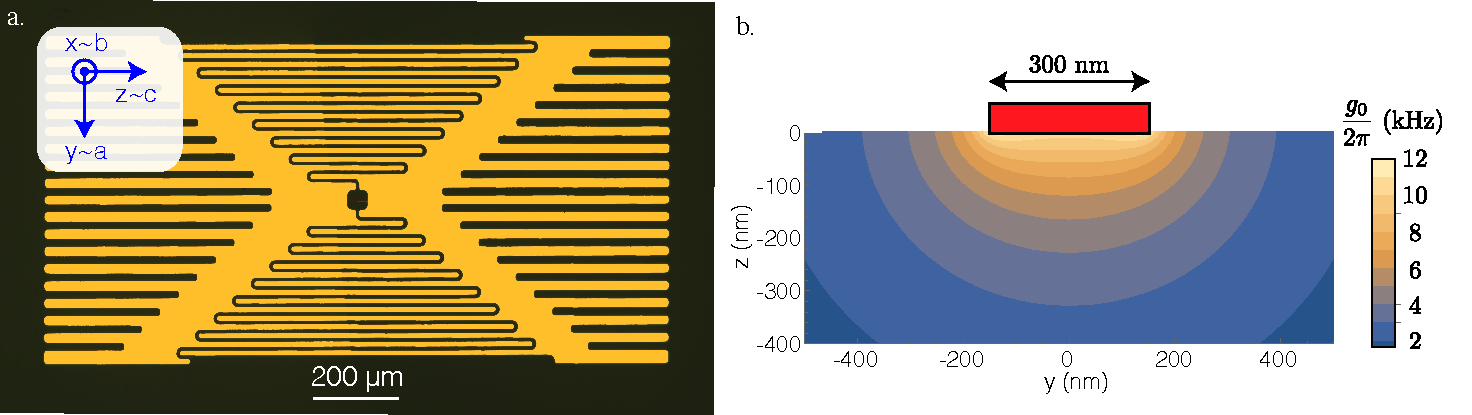
\includegraphics{chapter2/figures/sample.pdf}
    \caption[Sample micrograph and coupling map]{Sample micrograph and coupling map. \textbf{a.} False color micrograph of a Nb thin-film resonator of the same design fabricated on a \Ca crystal. The nanowire is colored in red while the rest of the resonator is colored yellow. The picture is stitched from 2 independent images. 
    \textbf{b.} Spatial map for the coupling g0 between the Er3+ and the superconducting resonator calculated with COMSOL. The map is shown as a transversal cut around the nanowire (in red).}
    \labfig{sample}
\end{figure*}

\subsection{The effect of the environment: losses and the Purcell effect}

We have considered the system of a resonator coupled to a spin isolated from the environment. In reality, both interact with the outside world in ways that are not tractable through unitary Hamiltonian evolution and require a more indirect approach. These external degrees of freedom effectively induce energy losses on both the resonator and the spin, as shown in \reffig{resonator_spin_lines}. The resonator can lose energy into the dielectric at a rate $\kappa_i$ and is capacitively coupled to microwave transmission lines, with which it exchanges energy at a rate $\kappa_c$. Therefore, the total loss rate of the resonator is $\kappa = \kappa_i + \kappa_c$. \sidenote{We say the resonator is overcoupled when the total loss is dominated by the capacitive coupling ($\kappa_c>\kappa_i$), undercoupled when the internal damping dominates ($\kappa_c<\kappa_i$), and critically coupled when they are balanced ($\kappa_c=\kappa_i$).} The spins, on the other hand, can spontaneously decay into the lattice via phonons. The non-radiative decay rate for \Er:\Ca at 10~mK is $\Gamma_\text{NR}/2\pi \approx 200$~kHz \sidecite{ledantec_electron_2022} and the surrounding magnetic environment induces decoherence at a rate $\Gamma_2$.

\begin{figure}
    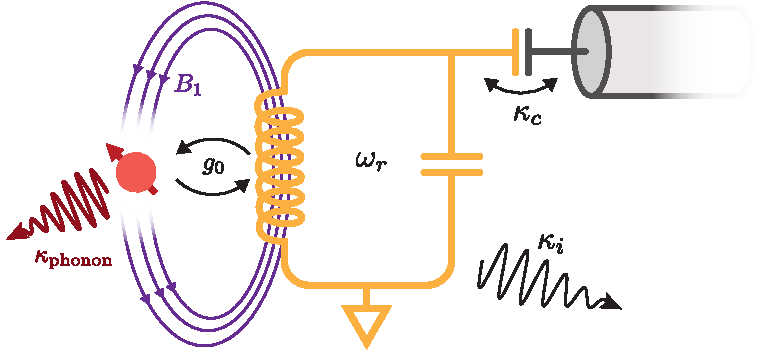
\includegraphics{chapter2/figures/resonator_spin_lines.pdf}
    \caption[Resonator coupled to a spin]{Resonator inductively coupled to a single electron spin. The resonator has two loss mechanisms: internal losses $\kappa_i$ and energy exchange with the capacitively coupled lines $\kappa_c$ and interacts with a spin with coupling strength $g_0$. The spin can decay via phonon relaxation with a rate $\kappa_\text{phonon}$}
    \labfig{resonator_spin_lines}
\end{figure}

Depending on the relative magnitude of the coupling $g_0$ and the relevant loss rates, two regimes can be distinguished.

\begin{itemize}
    \item \textit{Strong coupling regime}: $g_0 \gg \kappa, \Gamma_2$, where the system coherently exchanges excitations between the spin and the resonator multiple times before dissipating.
    \item \textit{Weak coupling regime}: $g_0 \ll \kappa, \Gamma_2$, where energy is damped before any coherent oscillations can occur.
\end{itemize}

The as measured in \refch{sample_and_setup}, the total losses of the resonator used in this work are $\kappa/2\pi \approx 700$~kHz. By comparing the losses to the expected coupling to the spins $g_0/2\pi \approx 10$~kHz $\ll \kappa$ we conclude we are deep in the weak-coupling regime. Nevertheless, the resonator enhances the density of states at the resonant frequency therefore boosting the radiative decay rate of any resonant \Er spin via the Purcell effect \sidecite{purcell_resonance_1946}. The Purcell radiative relaxation rate\sidenote{An in-depth derivation of the Purcell effect can be found in \cite{haroche_exploring_2006}.} is given by

\begin{equation}
\label{eq:Purcell_formula}
    \Gamma_\text{R}(\omega_S) = \frac{g_0^2\kappa}{(\omega_r-\omega_S)^2 + \kappa^2/4}.
\end{equation}

\noindent Moreover, the spin it undergoes a frequency shift (the Lamb shift)

\begin{equation}
\Delta\omega(\omega_S) = (\omega_r-\omega_S)\, \frac{g_0^2}{(\omega_r-\omega_S)^2 + \kappa^2/4}.
\end{equation}

At exact resonance ($\omega_r=\omega_S$) the shift vanishes and the Purcell rate is given by $\Gamma_\text{R}=4g_0^2/\kappa$, and the corresponding Purcell-limited lifetime is $\tau_P = 1/\Gamma_{S}$. Using the parameter estimates above gives $\Gamma_\text{R}\sim10^3\ \mathrm{s}^{-1}$, which is several orders of magnitude larger than the intrinsic phonon-limited relaxation. Consequently, the main relaxation path for resonant \Er spins becomes radiative.

The resulting photons can either be dissipated due to material losses in the substrate or sent to the coupled microwave lines, depending on the ratio between the $\kappa_i$ and $\kappa_c$. As demonstrated in previous work the optimal ratio for single photon detection is $\kappa_i = \kappa_c$ \sidecite{wang_addressing_2023} which are approximately the conditions achieved for this thesis (see \refsec{sample_details}).

\subsection{Controlling the state of the \Er ion}
\labsec{rabi_oscillations_theory}

In this section, we derive how a coherent drive on the resonator induces Rabi oscillations of the spin which naturally reveals the role of the cavity as a Lorentzian filter. We begin by considering the Jaynes-Cummings Hamiltonian, where the resonator is under the effect of a drive with complex amplitude $\epsilon_d$ and frequency $\omega_d$

\begin{equation}
    \frac{\cH{JC}}{\hbar} = \omega_r\,\hat{a}^\dagger \hat{a} +  \frac{\omega_S}{2} \hat{\sigma}_z + g_{0} ( \hat{a}\hat{\sigma}_{+} + \hat{a}^{\dagger}\hat{\sigma}_{-} ) + (\epsilon_d e^{-i\omega_d t} \hat{a}^\dagger + \epsilon_d^* e^{i\omega_d t} \hat{a}),
\end{equation}

Here we have dropped the factor $1/2$ from the resonator's energy and introduced the Pauli operators $S_i = \hbar / 2 \, \sigma_i$. In the rotating frame of the drive\sidenote{The unitary of the transformation is given by \[\hat{U}(t) = \exp{i\omega_d t \left(\hat{a}^\dagger \hat{a} +  \frac{1}{2} \hat{\sigma}_z \right)} \]} and applying the rotating wave approximation, the Hamiltonian becomes time independent and can be written as

\begin{equation}
    \frac{\cH{JC, R}}{\hbar} = \Delta_r\,\hat{a}^\dagger \hat{a} +  \frac{\Delta_S}{2} \hat{\sigma}_z + g_{0} ( \hat{a}\hat{\sigma}_{+} + \hat{a}^{\dagger}\hat{\sigma}_{-} ) + (\epsilon_d \hat{a}^\dagger + \epsilon_d^* \hat{a}),
\end{equation}

\noindent where $\Delta_r = \omega_r - \omega_d$ and $\Delta_S = \omega_S - \omega_d$. The driving term in the Hamiltonian will induce the cavity to develop a large coherent field $\alpha$ which translates as a non-zero photon occupation. From input-output theory \sidecite{blais_circuit_2020}, the equation of motion for the coherent state of the resonator under drive is given by  

\begin{equation}
    \dot{\alpha} = - \left( i\Delta_r + \frac{\kappa}{2}\right)\alpha - i\epsilon_d.
\end{equation}

For the steady state $\dot{\alpha}=0$, 

\begin{equation}
    \alpha = -\frac{\epsilon_d}{\Delta_r- i\kappa/2}.
\end{equation}

From this equation, we can see that the resonator beheaves as a Lorentzian filter: the coherent amplitude of the resonator is damped at large detunnings and broadened by $\kappa$. Given the non-zero cavity field, it is convinient to displace the Hamiltonian to be centered around $\alpha$ by introducing the displacement operator 

\begin{equation}
D(\alpha) = \exp\!\left(\alpha \hat{a}^\dagger - \alpha^* \hat{a}\right),
\end{equation}

which redefines the annihilation operator so that $\hat{a}$ describes only quantum fluctuations around the coherent amplitude. After the transformation the Hamiltonian becomes


\begin{equation}
    \frac{\cH{JC, R}'}{\hbar} = \Delta_r\,\hat{a}^\dagger \hat{a} +  \frac{\Delta_S}{2} \hat{\sigma}_z + g_{0} \left( (\hat{a} + \alpha)\hat{\sigma}_{x} + (\hat{a}^{\dagger} + \alpha^\dagger)\hat{\sigma}_{y} \right),
\end{equation}

By reorganizing terms we can distinguish three contributions:

\begin{align}
\begin{split}
    \frac{\cH{JC, R}'}{\hbar} = \underbrace{\Delta_r\,\hat{a}^\dagger \hat{a}}_\text{resonator} + \underbrace{\frac{\Delta_S}{2} \hat{\sigma}_z + g_{0} \left( \alpha\hat{\sigma}_{+} + \alpha^\dagger\hat{\sigma}_{-} \right)}_\text{spin} + \underbrace{g_{0} \left( \hat{a}\hat{\sigma}_{+} + \hat{a}^{\dagger}\hat{\sigma}_{-} \right)}_\text{coupling}.
\end{split}
\end{align}

If the amplitude of the coherent state is sufficiently large ($|\alpha|\gg1$) the coupling interaction between the resonator and the spin can be treated as a perturbation and the dynamics of the spin and the resonator can be disentangled. The resulting Hamiltonian for the spin is

\begin{equation}
    \frac{\cH{S, d}}{\hbar} = \frac{\Delta_S}{2} \hat{\sigma}_z + \frac{\Omega}{2} \left( \cos{\phi}\hat{\sigma}_{x} + \sin{\phi}\hat{\sigma}_{y} \right),
\end{equation}

\noindent where $\alpha = |\alpha| e^{i\phi}$ and $\Omega = 2g_0|\alpha|$. This corresponds to the classical two-level-system under drive and has an analytical solution.  If the spin is initially in the ground state, the excited-state population at time $t$ is


\begin{marginfigure}
    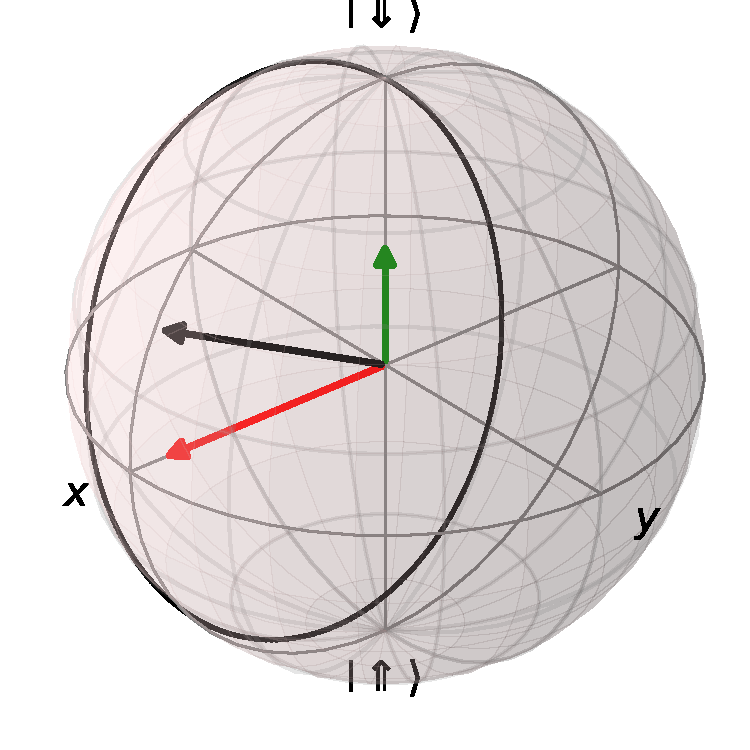
\includegraphics{chapter2/figures/qubit_dynamics.pdf}
    \caption[Spin dynamics]{Quantum trajectory of the spin in the Bloch sphere under a coherent drive. The detuning $\Delta_S$ and the drive $\Omega$ are represented as green and red arrows respectively and the resulting drive vector is plot in black. The trajectory is shown as a black curve.}
    \labfig{spin_trajectory}
\end{marginfigure}

\begin{equation}
    P_e(t) 
    = \frac{\Omega^2}{\Omega^2 + \Delta_S^2}\,
      \sin^2\!\left(\tfrac{1}{2}\sqrt{\Omega^2 + \Delta_S^2}\;t\right).
\end{equation}

At resonance ($\Delta_S=0$), this reduces to simple Rabi oscillations

\begin{equation}
    P_e(t) = \sin^2\!\left(\tfrac{\Omega}{2}\,t\right),
\end{equation}


with Rabi frequency $\Omega = 2g_0|\alpha| = 8g_0 \epsilon_d^2 / \kappa^2$, which grows as the square root of the mean intracavity photon number, $\Omega \propto \sqrt{\langle n \rangle}$. \reffig{spin_trajectory} shows the quantum trajectory of the spin in the Bloch sphere under the influence of a detuned drive with phase $\phi=0$. The state evolves from the ground state $\ket{\Downarrow}$ and is coherently excite. However, full population transfer to the excited state is only possible when $\Delta_S=0$.


\section[Detecting individual Er3+ ions through their fluorescence]{Detecting \Er ions through their fluorescence}
\labsec{Detecting_individual_Er}

\red{section is weak as fuck, improve and add graphs}

Single-electron spin sensitivity has been recently demonstrated in our group through the use of a unique device known as the Single Microwave Photon Counter (SMPD) \sidecite{wang_addressing_2023}. Unlike traditional single-spin readout methods that rely on spin-dependent optical fluorescence \sidecite{wrachtrup_optical_1993} or on transport-based spin-to-charge conversion (STM \sidecite{elzerman_singleshot_2004} or quantum-dot readout \sidecite{rugar_single_2004}), the SMPD operates entirely in the microwave regime and does not require system specific mechanisms like optical transitions or spin-to-charge conversion. 

The measurement is performed by monitoring the Purcell enhanced microwave fluorescence emission of the \Er ion. The detector  effectively behaves as a counter, mapping every incoming microwave photon within its bandwidth to a discrete event. In this thesis we treat the detector as black box which counts photons with efficiency $\eta_{d}$ and has an intrinsic noise floor defined by the dark counts rate $\Gamma_{DC}$. Appendix \ref{app:SMPD} describes the operation and characteristics of the device.
